%%% -*-LaTeX-*-

\chapter{The Multi-cluster Trading Mechanism}

As the adoption of multi-cluster environments accelerates and the
infrastructure continues to evolve to support more use-cases, we are presented
with an opportunity to build tools on top of that and leverage the existing
networking innovations to optimize how clusters interact in a multi-cluster
environment. Since a multi-cluster environment is a loose definition, we define
our multi-cluster environment as a one which clusters are discoverable to one
another and implements the trading mechanism's API.

We argue that it is possible to increase cluster resource utilization,
decrease average job completion time, and/or reduce average cost by providing
clusters with a resource trading mechanism allowing the virtual sharing of
resources across clusters. 

The trader is the component putting the mechanism in effect. It involves
receiving policies as input from the user, communicating with other clusters'
traders and facilitating the exchange of resources between them. It is the
point of contact between the foreign clusters and the host cluster's scheduler.

In this chapter we present the system design, discuss the role of the scheduler
in the mechanism, explain what user-defined policies are and lastly describe
the design of the trader itself. 

The next figure portrays an overview of the system:

\begin{figure}[H]
  \centerline{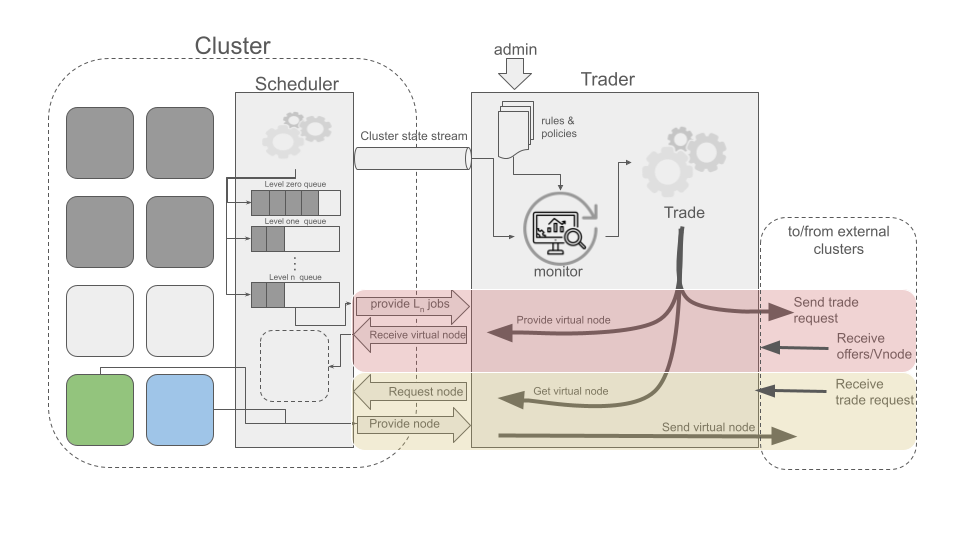
\includegraphics[scale=0.45]{figures/system-diagram}}
  \caption{System architecture showing the various compononents of the trader,
    and how it connects to a cluster. Red section represents the procedure
    requesting resources and the yellow section depicts the procedure of
    providing resources to external clusters. squares represents the node in
    the host cluster. Dark gray nodes represent localy utilized nodes and light
    gray nodes represent free local nodes. Green and blue nodes represent
    resources    provided to external clusters and the dotted square is a
    virtual node received from an external cluster} 
  \figlabel{fig1}
  \end{figure}


\section{Scheduler}
% introducing the notion of minimal intursivity
\subsection{Requirements}
Cluster scheduling have been widely studied and remains a prominent area of
research. Our objective in relation to scheduling is not to replace the
clusters' scheduling algorithm nor interfere with its scheduling decisions, but
to improve the cluster's performance while minimizing friction and interaction
with the trader. It it also worth noting that the scheduler does not directly
interact with the broader multi-cluster environment but only with its own
trader, reducing the communication surface area and keeping local scheduling
independent from the mechanism. [NEEDS BETTER WORDING]

The scheduler's role in the mechanism comprises of passing on cluster state to
local trader, providing resources for trades, and receiving resources from
trades. Cluster state are measurements necessary to inform trading decisions.
These metrics are typically collected in cluster schedulers for performance
analysis and monitoring and include wait time, cost of compute/memory,
utilization etc.

\noindent Providing and receiving resources are an extension of the cluster's
ability to add new nodes and allocate resources on existing ones. 

Thus scheduling is detached from trading and only an interface is required to
connect the two modules together, allowing any scheduling algorithm already
running in a cluster to remain unchanged. This lays the ground to the general
requirements for a scheduler to operate in the mechanism, and shows that a
specific scheduling algorithm is not required for our mechanism. With that
being said, we now present our scheduling algorithm and discuss the underlying
design decisions. 

\subsection{Design}
% delay scheduling 

The base of our scheduling algorithm is delay scheduling [CITE] due to its
simplicity and []focus on data locality. In delay scheduling, a job is first
assigned the lowest level 0, allowing it to only be scheduled on the node its
data is at. The job is subsequently bumbed to higher levels as it fails to get
it scheduled in close proximity, permitting the scheduler to schedule the job
further away from its data as the wait time of the job increases. Consequently
the leveling represent the job's expectated distance from its data. This notion
of proximity and gradual drifting[] is extended to include external clusters in
our mechanism. Jobs already anticipating poor data locality would be the ones
more likely to be scheduled on an external cluster. This insures fair
scheduling even as we extend the scope of scheduling to a multi-cluster
environment. These jobs would also incur the least percentage reduction in
performance when scheduled in a foreign cluster.

\figref{fig1} includes the architecture of the scheduler described here. The
different queues represent different levels a job can be in. The incoming and
outgoing arrows represents the exposed interface the trader utilize to
communicate with the scheduler and will be further explained in the trader
section \ref{trader}. 

%Of course, more analysis could go in deciding what jobs would better fit being
%exported to other clusters like jobs demanding less communiication with other
%jobs in the cluster, jobs with less data dependency, ..., but this is out of
%scope of this thesis.


% research idea: data locality-aware scheduling research is trying to get the
% jobs scheduled next to data, no study i encountered actually socres the
% sensitivity of the jobs in relation to other jobs in the cluster. (probably
% for fairness concerns) but might be an interesting project to work on. 

%This presents us with a clean heuristic when calculalting resources needed for
%trading. As the level of the of what to include in our 

\section{Policies}

% Policy intro
Policies are created to optimize a specific performance metric, acting as knobs
to tune the mechanism and update it as cluster requirements change. They are a
set of rules that dictate how each cluster handles trading. Policies are
pluggable and mutable, meaning each cluster can implement its own request and
receive policy, and dynamically update it as requirements or conditions change.
Policies are two types, incoming and outgoing. 

\subsection{Incoming} 

Incoming policies set the rules for accepting resource requests from foreign
clusters. The mechanism consults the policy, comparing the current cluster
state with the requested resources and concludes its decision.

% add figure for policy? or give an example??
[ADD FIGURE]

\subsection{Outgoing}

As the system continously monitors the cluster state, it makes sure the state
does not break any of the outgoing policies' requirements. Once that happens
the mechanism initiates the trading procedure. 

[ADD FIGURE]

\section{Trader}

The trader is the main component of the mechanism. As an orchestrator, K8s role
is to sync the actual cluster state with the declared desired state. This
involves spawning a new container if an old one died or scaling a service if it
gets more traffic. The trader plays a similar role, it is responsible for
keeping the cluster's state in sync with the declared desired state. The
desired state is declared through the user defined outgoing policies. Once the
current state of the cluster breaks an outgoing policy, it initiates the
trading request algorithm. 
% add trading request algorithm
% Example Algorithm
\begin{algorithm}[H]
\caption{Trading Scheduling Algorithm - Requester}
\begin{algorithmic}
    \For{job in WaitQueue}
        \State $scheduled \gets ScheduleJob(job)$
        \If{$scheduled \neq True$ \&\& Policy(job) $==$ True} 
        \State $requestResources(job)$
        \EndIf
    \EndFor

    \For{job in ReadyQueue}
        \State $scheduled \gets ScheduleJob(job)$
        \If{$scheduled \neq True$}
        \State $WaitQueue \gets WaitQueue + job$
        \EndIf
    \EndFor
\end{algorithmic}
\end{algorithm}

The first step in the trading algorithm is determining the amount of resources
needed. First, the trader requests more information from the scheduler. The
scheduler is required to share a job's list with the trader. The trader in turn
uses the information provided to calculate the requested node size. The user
defined outgoing policy also dictates any additional constraints the trader is
required to adhere to. If the notion of a currency is established in the
multi-cluster environmnet, constraints would include a budget, as well as a
maximum price to pay for resources, which can be the price of renting out the
resources from the vendor, or a cost estimate anaylsis algorithm. 

After calculating the needed resources, the trader then broadcasts a contract
to all participating clusters, and waits for replies. After receiving approved
contracts, the trader approves the best contract, and receives the virtual node
information from the foreign trader. It then sends the virtual node for the
scheduler to start scheduling jobs on it.

\begin{algorithm}[H]
    \caption{Trading Scheduling Algorithm - Receiver}
    \begin{algorithmic}
            \State $ resources \gets BorrowRequest $ \Comment{Incoming from another cluster} 
            \If{$Policy(resources) = True$} 
            \State $sendAcceptRequest(job, cluster)$
            \State $prepareResources(resources)$
            \State $allowAccess$
            \EndIf
    \end{algorithmic}
\end{algorithm} 

The trader is also responsible for accepting/rejecting incoming requests. After
receiving a contract request, the trader consults the incoming policy and the
current cluster state, and decides whether to approve the contract. If the
trader gets picked by the foreign cluster, the trader then requests the needed
resources from the scheduler and sends the node information back to the foreign
trader.
%Our mechanism offers bidirectional trading, allowing clusters to trade
%resources with one another. It also enables trading with multiple clusters, so
%clusters can trade resources with more than one cluster at a time.
%\label{sched-overhead} The following algorithms show a simple representation
%of the system, with resource utilization as the optimized-for metric:
%\label{example}
